\section{Systembeskrivelse}
Der ønskes at udvikle et system, der har til formål at aflaste musklerne omkring knæleddet under udførelse af en squat i statisk bevægelse ved brug af body augmentaion. Da ALS-patienter efterhånden mister kræften i musklerne, grundet neurodegenerativ, vil det ved brug af et exoskelet være muligt at aflaste patienterne, med henblik på at kunne undgå kørestol i et tidligere stadie. Systemet skal kunne opsamle signaler fra lårmusklerne, quadriceps og hamstring. Denne aktivitet skal omsættes til exoskelettet som skal udføre en tilsvarende bevægelse. Udover aktiviteten i musklerne skal exoskelettet have et input, som begrænser, bevægelse i forskellige retninger, herved er det muligt at rette leddet, hvis patienten kommer ud af den ønskede position. Derfor skal systemet være i stand til at måle muskelaktivitet og acceleration. Derudover skal produktet være brugervenligt ved, at være kompakt, mobilt og ikke generende over for brugeren.

\subsection{Krav til systemet} 
\fxnote{Er der andre krav i mener vi mangler?}
\begin{itemize}
\item Systemet skal registrere muskelaktivitet og acceleration
\item Systemet skal være batteridrevet
\item Systemet skal kunne give feedback, hvis der ikke er strøm nok til at virke optimalt
\item Systemet skal ikke være til gene for brugeren
\item Systemet skal kunne overføre data til en trådløs computer
\item Systemet skal kunne give feedback og derved sørge for at brugeren befinder sig inden for følgende specifikationer:
\begin{itemize}
\item XX antal grader?
\item XX antal grader?
\end{itemize}
\end{itemize}


\subsection{Blokdiagram}
\begin{figure}[H]
\centering
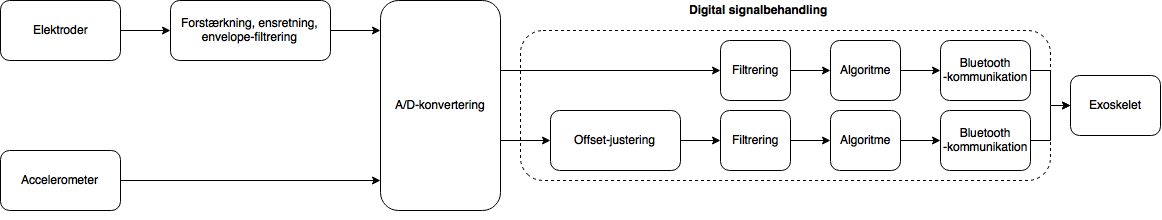
\includegraphics[width=0.4\textwidth]{figures/blokdiagram.png}
\caption{Blokdiagram over systemets opbygning}
\label{fig:blokdiagram}
\end{figure}

I dette projekt er der valgt at udarbejde en prototype, som har til formål at sørge for at knæledddet forbliver inden for en bestemt position. Opbygningen af systemet fremgår af \autoref{fig:blokdiagram}. Der anvendes to sensorer til at opsamle signaler herunder EMG og accelerometer. For at registrere muskelaktivitet anvendes en EMG-forstærker, der har til formål at forstærke den muskelaktivitet som opsamles. Acceleration anvendes for at give et input om hvor knæet befinder sig under udøvelsen af en statisk squat. Det opsamlede signal sendes videre til den digitale del bestående af et Bluetooth Low Energy Pioneer kit (CY8CKIT-042-BLE)som opfanger signalet og overfører signalet trådløst til en CySmartUSB BLE Dongle. 

